\documentclass[a4paper, 12pt]{report}
\usepackage[utf8]{inputenc}
\usepackage[T1]{fontenc}

\usepackage{xcolor}
\usepackage{afterpage}

\usepackage{relsize}
\usepackage{moresize}

\usepackage{graphicx}
\usepackage{geometry}

% [CHANGE] The title of your thesis. If your thesis has a subtitle, then this
% should appear right below the main title, in a smaller font.
\newcommand{\theTitle}{Efficient Semifield Convolutions}
\newcommand{\theSubTitle}{}


% [CHANGE] Your full name. In case of multiple names, you can include their
% initials as well, e.g. "Robin G.J. van Achteren".
\newcommand{\theAuthor}{Peter Adema}

% [CHANGE] Your student ID, as this has been assigned to you by the UvA
% administration.
\newcommand{\theStudentID}{14460165}

% [CHANGE] The name of your supervisor(s). Include the titles of your supervisor(s),
% as well as the initials for *all* of his/her first names.
\newcommand{\theSupervisor}{Dr.\ ir.\ R.\ van den Boomgaard} % Dr. Ing. L. Dorst

% [CHANGE] The address of the institute at which your supervisor is working.
% Be sure to include (1) institute (is appropriate), (2) faculty (if
% appropriate), (3) organisation name, (4) organisation address (2 lines).
\newcommand{\theInstitute}{
Informatics Institute \\ %Institute for Logic, Language and Computation
Faculty of Science\\
University of Amsterdam\\
Science Park 900 \\ 
1098 XH Amsterdam 
}

% [CHANGE] The semester in which you started your thesis.
\newcommand{\theDate}{Semester 2, 2024-2025}



\usepackage[shortlabels]{enumitem}
\usepackage{graphicx}

\usepackage{hyperref}
\usepackage{amsmath}
\usepackage{amssymb}
\usepackage{amsthm}
\usepackage{mathabx}
%\usepackage{apacite}
\usepackage{caption}
\usepackage{listings}
\usepackage{xcolor}
\usepackage{array}
\usepackage{booktabs}
\def\comment#1{\color{red}#1\color{black}}
\usepackage{bbold}
\DeclareMathOperator{\boxclose}{\vcenter{\hbox{$\blacksquare$}}}
\DeclareMathOperator{\boxopen}{\Box}
\definecolor{opening_red}{RGB}{169,15,70}
\definecolor{opening_blue}{RGB}{94, 79, 162}
\begin{document}
\pagestyle{empty}
\begin{center}

\vspace{2.5cm}


\begin{Huge}
% see definition at beginning of document
\theTitle
\end{Huge} \\

\vspace{0.5 cm}

\begin{Large}
\theSubTitle
\end{Large}

\vspace{1.5cm}

% see definition at beginning of document
\theAuthor\\
% see definition at beginning of document
\theStudentID

\vspace{1.5cm}

% [DO NOT CHANGE]
Honours Thesis extension\\
Credits: 6 EC

\vspace{0.5cm}

% [DO NOT CHANGE] The name of the educational programme.
Bachelor \textit{Kunstmatige Intelligentie} \\
\vspace{0.25cm}
\includegraphics[width=0.075\paperwidth]{figures/uva_logo} \\
\vspace{0.1cm}

% [DO NOT CHANGE] The address of the educational programme.
University of Amsterdam\\
Faculty of Science\\
Science Park 900\\
1098 XH Amsterdam

\vspace{2cm}

\emph{Supervisor}\\

% see definition at beginning of document
\theSupervisor

\vspace{0.25cm}

% see definition at beginning of document
\theInstitute

\vspace{1.0cm}

% see definition at beginning of document
\theDate

\end{center}
\newpage



\pagenumbering{arabic}
\setcounter{page}{1}
\pagestyle{plain} 


\section*{Abstract \comment{TODO}}


\section*{Acknowledgements \comment{TODO}}

\newgeometry{a4paper, textwidth=400.0pt, textheight=740.0pt}
\tableofcontents


\chapter{Introduction \comment{TODO}}


\newpage
\section{Related work \comment{TODO}}


\chapter{Convolutional derivatives}
To perform semifield convolutions within the context of a deep-learning application, we must ensure that we can take the gradient with respect to our inputs in an efficient manner for all operations we seek to perform. 
The primary challenge in this case is not necessarily the gradient for $\otimes$, as this is a scalar function applied once within each path in the computational graph. Instead, the challenge lies in calculating the derivative of the semifield summation $\bigoplus$, as all terms within this reduction could influence the gradient of all others. While it would be possible to simply perform backpropagation through every instance of $\oplus$ separately, this would be very computationally expensive and likely numerically unstable. As such, we would like to define semifield operators for the cases when we can find a more efficient method to calculate the derivative of $\oplus$.

We have identified three cases in which this is possible, and will discuss them in order of increasing implementation complexity. First, we will examine the possibility of using operators provided by PyTorch to implement semifield convolutions. Afterwards, we will show the two common cases for which a reduction has a simple analytical derivative, namely for those operators $\oplus$ which act like $\max$, and those which are invertible.

\section{PyTorch reduction operators}
The most straight-forward method for implementing semifield convolutions for PyTorch models is clearly to use reduction operators provided by PyTorch itself. These operators have their derivatives provided by PyTorch, and are integrated into the PyTorch automatic differentiation system such that writing a backward pass is not required.

The challenge when using PyTorch operators lies then not in their derivative, but in how to apply them in the correct fashion: the axes we would wish to reduce over are not the image axes present in the input itself, but instead the window axes of every sliding window we extract during the convolution.

A built-in method for accomplishing this is \verb nn.Unfold , an operator which examines sliding windows from the input and copies each separately to a new buffer, allowing subsequent operators to work with the window axes of the new buffer. This copying is rather suboptimal, however: if we take a relatively small $32\times32$ image and extract relatively small $5\times5$ windows from it, then the result is more than 19 times the size of the image: even ignoring the cost of copying, larger inputs or kernel sizes would quickly lead to memory issues.

As such, we would wish to perform a similar operation (transforming the input image such that we have access to sliding window axes to reduce over), but without performing a copy. This is possible by creating an adjusted view of the input image: some other libraries include this feature by default, but it is not exceedingly complex to replicate.

The main idea of using such a view is to adjust the strides (step sizes within the underlying data array) such that, when moving to the next window, the view takes a step equal to the convolutional $\textsc{stride}$ instead of the full size of the window. In Fig. \ref{fig:strides}, we can see how a view into a 1D-array with $\textsc{stride}=1$ and size-4 kernels causes subsequent windows to overlap:

\begin{figure}[ht!]
	\center
  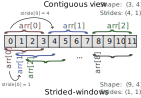
\includegraphics[width=1\textwidth]{extension-figures/strides.png}
  \caption{Two views onto the same underlying data: at the top, a contiguous view (the typical view for PyTorch arrays), and at the bottom, a strided-windows view (allowing for extracting windows without copying). }
  \label{fig:strides}
\end{figure}

\noindent
By applying a broadcasting version of $\otimes$ to the strided view and the convolutional kernels, we can obtain the intermediaries to be reduced.
By applying the reduction operator along the window axis (axis 1 in Fig. \ref{fig:strides}), we can then efficiently calculate $\bigoplus$ for all cases where $\bigoplus$ and $\otimes$ can be expressed as one or more PyTorch operators.

However, this approach still has a major downside in terms of memory usage and cache locality: there is currently no method for fusing the $\otimes$ and $\bigoplus$ operations in PyTorch, and the intermediary results of $\otimes$ must therefore be manifested in their entirety. As a result, this method still suffers from greatly increased memory use but  (more importantly for the small-scale experiments in the main report) also accesses memory inefficiently. Since all results of $\otimes$ are stored an calculated before $\bigoplus$ begins, the initial results of $\otimes$ are flushed from the cache by the beginning of $\bigoplus$, causing further slowdowns from cache-misses.

In order to mitigate this, we must devise custom, fused kernels that combine $\otimes$ and $\bigoplus$ into a single operation. This, however, also requires calculating the derivative rules manually; the next two sections will discuss two such rulesets.

\section{Selection-based semifield addition \comment{TODO}}
If it acts like $\max$, we can memoize the provenance (which value was selected).
\section{Invertible semifield addition \comment{TODO}}
If we can undo it, we can use \cite{ppad}.

\chapter{CUDA semifield convolutions \comment{TODO}}
Armed with an understanding of the types of semifield convolutions where a gradient can be calculated in a reasonably efficient manner, we now turn to the task of efficiently implementing these operations as programs that can run on a (NVIDIA) GPU: CUDA kernels.

\chapter{PyTorch C++ Extensions \comment{TODO}}
Now that we have working implementations of semifield convolutions in the form of CUDA kernels, it is important to examine how these kernels can best be used within the context of a deep-learning model created with the PyTorch machine learning framework.

\chapter{Conclusions \comment{TODO}}

\section{Findings \comment{TODO}}
\section{Discussion \comment{TODO}}

\newpage
\section{Contributions \comment{TODO}}
\section{Further research \comment{TODO}}

\section{Reproducibility \comment{TODO}}
\section{Ethics \comment{Maybe?}}
\comment{\ldots\ldots}

%\newgeometry{a4paper, textwidth=400.0pt, textheight=770.0pt}
\bibliographystyle{IEEEtran}
{\footnotesize \bibliography{references}}
%\newgeometry{a4paper, textwidth=400.0pt, textheight=740.0pt}

\newpage
\chapter{Appendix}

\end{document}
